\paragraph{Activité~4} Zellige\\

Cette activité consiste à étudier l'enchaînement de deux translations sur un damier de carreaux Zellige, un carrelage décoratif originaire de l'Antiquité Méditerranéenne et du Moyen Orient.\\

\begin{tikzpicture}[scale=0.45,line cap=round,line join=round,>=triangle 45,x=1.0cm,y=1.0cm]
\pgfmathsetmacro{\nbSurY}{7}
\pgfmathsetmacro{\nbSurX}{6}
%
\pgfmathsetmacro{\YY}{(\nbSurY - 1) * 4}
\pgfmathsetmacro{\XX}{(\nbSurX - 1) * 4}
\pgfmathsetmacro{\grilleYY}{(\nbSurY + 1) * 4 - 1}
\pgfmathsetmacro{\grilleXX}{(\nbSurX + 1) * 4}


\grille{0}{0}{\grilleXX}{\grilleYY}{help lines}
%\foreach \y in {0, 4, 8, ..., \YY}{
%%\pgfmathsetmacro{\Y}{\y}
%	\foreach \x in {0, 4, 8, ..., \XX}{
%%	\pgfmathsetmacro{\X}{\x}
%	\pgfmathsetmacro{\numero}{(0.25*(\y*6+\x)+1)}
%		\begin{scope}[shift={(\x cm, \y cm)}]
%		\placerpointsansnom{A}{4}{6}{above left};
%		\placerpointsansnom{B}{5}{5}{above right};
%		\placerpointsansnom{C}{7}{5}{above right};
%		\placerpointsansnom{D}{5}{3}{above left};
%		\placerpointsansnom{E}{6}{1}{below right};
%		\placerpointsansnom{F}{5}{1}{below left};
%		\placerpointsansnom{G}{4}{2}{above left};
%		\placerpointsansnom{H}{3}{1}{below right};
%		\placerpointsansnom{I}{2}{1}{below left};
%		\placerpointsansnom{J}{1}{3}{above left};
%		\placerpointsansnom{K}{3.5}{3.5}{above left};
%			\fill[lightgray] (K) circle(1);
%			\draw (K) node {\pgfmathprintnumber{\numero}};
%			\draw[very thick] (A)--(B)--(C)--(D)--(E)--(F)--(G)--(H)--(I)--(J)--cycle;
%		\end{scope}
%	}
%}
%\vectAuColor{r}{18}{1}{4}{4}{4pt}{-0.1}{below}{red};
%\vectAuColor{s}{19}{29}{8}{0}{4pt}{1}{right}{red};
%\vectAuColor{t}{14}{5}{0}{-4}{4pt}{1.1}{below}{red};
\vectAuColor{u}{1}{15}{12}{-8}{4pt}{0}{left}{blue};
\vectAuColor{v}{10}{5}{-4}{-4}{4pt}{1.1}{below}{cyan};
%\vectAuColor{w}{9}{25}{12}{-4}{4pt}{0.4}{above}{red};


% Carreau 26
\begin{scope}[shift={(4 cm, 16 cm)}]
	\placerpointsansnom{A}{4}{6}{above left};
	\placerpointsansnom{B}{5}{5}{above right};
	\placerpointsansnom{C}{7}{5}{above right};
	\placerpointsansnom{D}{5}{3}{above left};
	\placerpointsansnom{E}{6}{1}{below right};
	\placerpointsansnom{F}{5}{1}{below left};
	\placerpointsansnom{G}{4}{2}{above left};
	\placerpointsansnom{H}{3}{1}{below right};
	\placerpointsansnom{I}{2}{1}{below left};
	\placerpointsansnom{J}{1}{3}{above left};
	\placerpointsansnom{K}{3.5}{3.5}{above left};
	\fill[green] (K) circle(1);
	\draw[black] (K) node {\textbf{26}};
	\draw[green,ultra thick] (A)--(B)--(C)--(D)--(E)--(F)--(G)--(H)--(I)--(J)--cycle;
\end{scope}

% Carreau 17
\begin{scope}[shift={(16 cm, 8 cm)}]
	\placerpointsansnom{A}{4}{6}{above left};
	\placerpointsansnom{B}{5}{5}{above right};
	\placerpointsansnom{C}{7}{5}{above right};
	\placerpointsansnom{D}{5}{3}{above left};
	\placerpointsansnom{E}{6}{1}{below right};
	\placerpointsansnom{F}{5}{1}{below left};
	\placerpointsansnom{G}{4}{2}{above left};
	\placerpointsansnom{H}{3}{1}{below right};
	\placerpointsansnom{I}{2}{1}{below left};
	\placerpointsansnom{J}{1}{3}{above left};
	\placerpointsansnom{K}{3.5}{3.5}{above left};
	\fill[blue] (K) circle(1);
	\draw[white] (K) node {\textbf{17}};
	\draw[blue,ultra thick] (A)--(B)--(C)--(D)--(E)--(F)--(G)--(H)--(I)--(J)--cycle;
\end{scope}

% Carreau 1
\begin{scope}[shift={(12 cm, 4 cm)}]
	\placerpointsansnom{A}{4}{6}{above left};
	\placerpointsansnom{B}{5}{5}{above right};
	\placerpointsansnom{C}{7}{5}{above right};
	\placerpointsansnom{D}{5}{3}{above left};
	\placerpointsansnom{E}{6}{1}{below right};
	\placerpointsansnom{F}{5}{1}{below left};
	\placerpointsansnom{G}{4}{2}{above left};
	\placerpointsansnom{H}{3}{1}{below right};
	\placerpointsansnom{I}{2}{1}{below left};
	\placerpointsansnom{J}{1}{3}{above left};
	\placerpointsansnom{K}{3.5}{3.5}{above left};
	\fill[cyan] (K) circle(1);
	\draw[black] (K) node {\textbf{10}};
	\draw[cyan,ultra thick] (A)--(B)--(C)--(D)--(E)--(F)--(G)--(H)--(I)--(J)--cycle;
\end{scope}

\vectAuColor{u}{11}{21}{12}{-8}{4pt}{0.1}{above right}{blue};
\vectAuColor{u}{5}{19}{12}{-8}{4pt}{0.5}{above right}{blue};
%\vectAuColor{u}{8}{22}{12}{-8}{4pt}{0}{above}{purple};

\vectAuColor{v}{23}{13}{-4}{-4}{4pt}{0.2}{below right}{cyan};
\vectAuColor{v}{17}{11}{-4}{-4}{4pt}{0.5}{above left}{cyan};
%\vectAuColor{v}{20}{14}{-4}{-4}{4pt}{0.5}{above left}{purple};

\draw[->,>=latex,line width=4pt,purple] (5,19) -- (13,7) node[fill=white,pos=0.3,below left] {$\textcolor{purple}{\overrightarrow{u} + \overrightarrow{v}}$};
\draw[->,>=latex,line width=4pt,purple] (5,19) -- (13,7); % On retrave le vecteur sur l'étiquette du nom

\end{tikzpicture}



\newpage

\begin{enumerate}
	\item Enchaînement 1
	\vspace{-2em}
		\begin{enumerate}
			\item Quelle est l'image du carreau \zellige{26} par la translation de vecteur \vectaffiche{u}~? \textcolor{blue}{C'est le carreau 17.}
			\item Quelle est l'image de cette image par la translation de vecteur~\vectaffiche{v}~?
				 \textcolor{cyan}{C'est le carreau 10.}
			\item Émettre une conjecture sur la nature de la transformation correspondant à l'enchaînement de ces deux translations.
				 \textcolor{purple}{C'est la translation de vecteur \vectaffiche{u} suivie de la translation de vecteur \vectaffiche{v}.}
		\end{enumerate}
\end{enumerate}
\begin{center}
	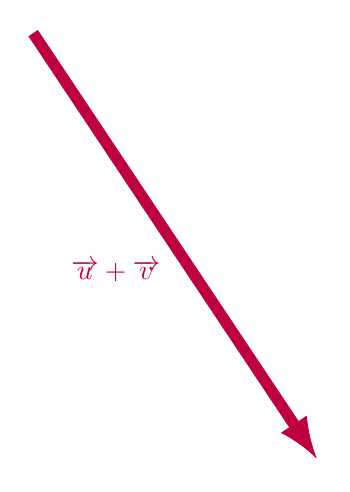
\begin{tikzpicture}[scale=0.45,every node/.style={scale=1}]
		\vectAuColor{u}{5}{19}{12}{-8}{4pt}{0.5}{above right}{blue};
		\vectAuColor{v}{17}{11}{-4}{-4}{4pt}{0.5}{above left}{cyan};
		\draw[->,>=latex,line width=4pt,purple] (5,19) -- (13,7) node[fill=white,pos=0.5,below left] {$\textcolor{purple}{\overrightarrow{u} + \overrightarrow{v}}$};
		\draw[->,>=latex,line width=4pt,purple] (5,19) -- (13,7); % On retrave le vecteur sur l'étiquette du nom
	\end{tikzpicture}
	\fbox{On notera \textcolor{purple}{\vectaffiche{u} + \vectaffiche{v}} les caractéristiques de cette nouvelle transformation}
\end{center}
	
\begin{enumerate}
	\setcounter{enumi}{1}
	\item Enchaînement 2
	\vspace{-2em}
		\begin{enumerate}
			\item Quelle est l'image du carreau \zellige{38} par la translation de vecteur \vectaffiche{s}~? \textcolor{red}{C'est le carreau 40.}
			\item Quelle est l'image de cette image par la translation de vecteur~\vectaffiche{t}~?
				 \textcolor{red}{C'est le carreau 34.}
			\item Émettre une conjecture sur \vectaffiche{s} + \vectaffiche{t}. \textcolor{red}{C'est la translation de vecteur \vectaffiche{s} suivie de la translation de vecteur \vectaffiche{t}.}
		\end{enumerate}
	\item Enchaînement 3
	\vspace{-2em}
		\begin{enumerate}
			\item Quelle est l'image du carreau \zellige{22} par la translation de vecteur \vectaffiche{v}~? \textcolor{red}{C'est le carreau 15.}
			\item Quelle est l'image de cette image par la translation de vecteur~\vectaffiche{r}~?
				 \textcolor{red}{C'est le carreau 22.}
			\item Émettre une conjecture sur \vectaffiche{v} + \vectaffiche{r}. \textcolor{red}{On revient sur le carreau de départ. \vectaffiche{v} + \vectaffiche{r} est le vecteur nul :  \vectaffiche{v} + \vectaffiche{r} $=$ \vectaffiche{0}.}
		\end{enumerate}
\end{enumerate}